\chapter{Minimalflächen\label{chapter:thema}}
\lhead{Minimalflächen}
\begin{refsection}
\chapterauthor{Nadja Rutz und Ambroise Suter}

\section{Einleitung}
\rhead{Einleitung}
Was sind Minimalflächen? 
Wie werden sie definiert? 
Warum passen sie in den Kontext dieses Buches?
Diese Fragestellungen werden im Laufe dieses Kapitel an Hand von Beispielen illustriert und erörtert.

Wie der Name erahnen lässt beschreiben Minimalflächen Flähen mit minimalem Flächeninhalt. 
Ein gängiges Beispiel aus der Physik sind Seifenfilme. Wenn die Luft auf beiden Seiten eines Seifenfilms den gleichen Druck hat, dann ist er eine Minimalfläche.


\section{Katenoid}
\rhead{Katenoid}
Wenn man zwei koaxiale Drahtringe parallel zueinander in Seifenwasser taucht, entsteht eine Rotationsfläche (Abbildung \ref{KatenoidSeifenfilm}) welche Katenoid genannt wird. 

Das Katenoid ist die erste entdeckte Minimalfläche.
Sie wurde schon 1776 von Jean Baptiste Meusnier erstmals beschrieben.
In diesem Abschnitt wird die mathematische Herleitung des Katenoids mit Hilfe der Eulerschen Differenzialgleichung der Variationsrechnung aufgezeigt.
\subsection{Beispiel Katenoid}

\begin{figure}
  \centering
  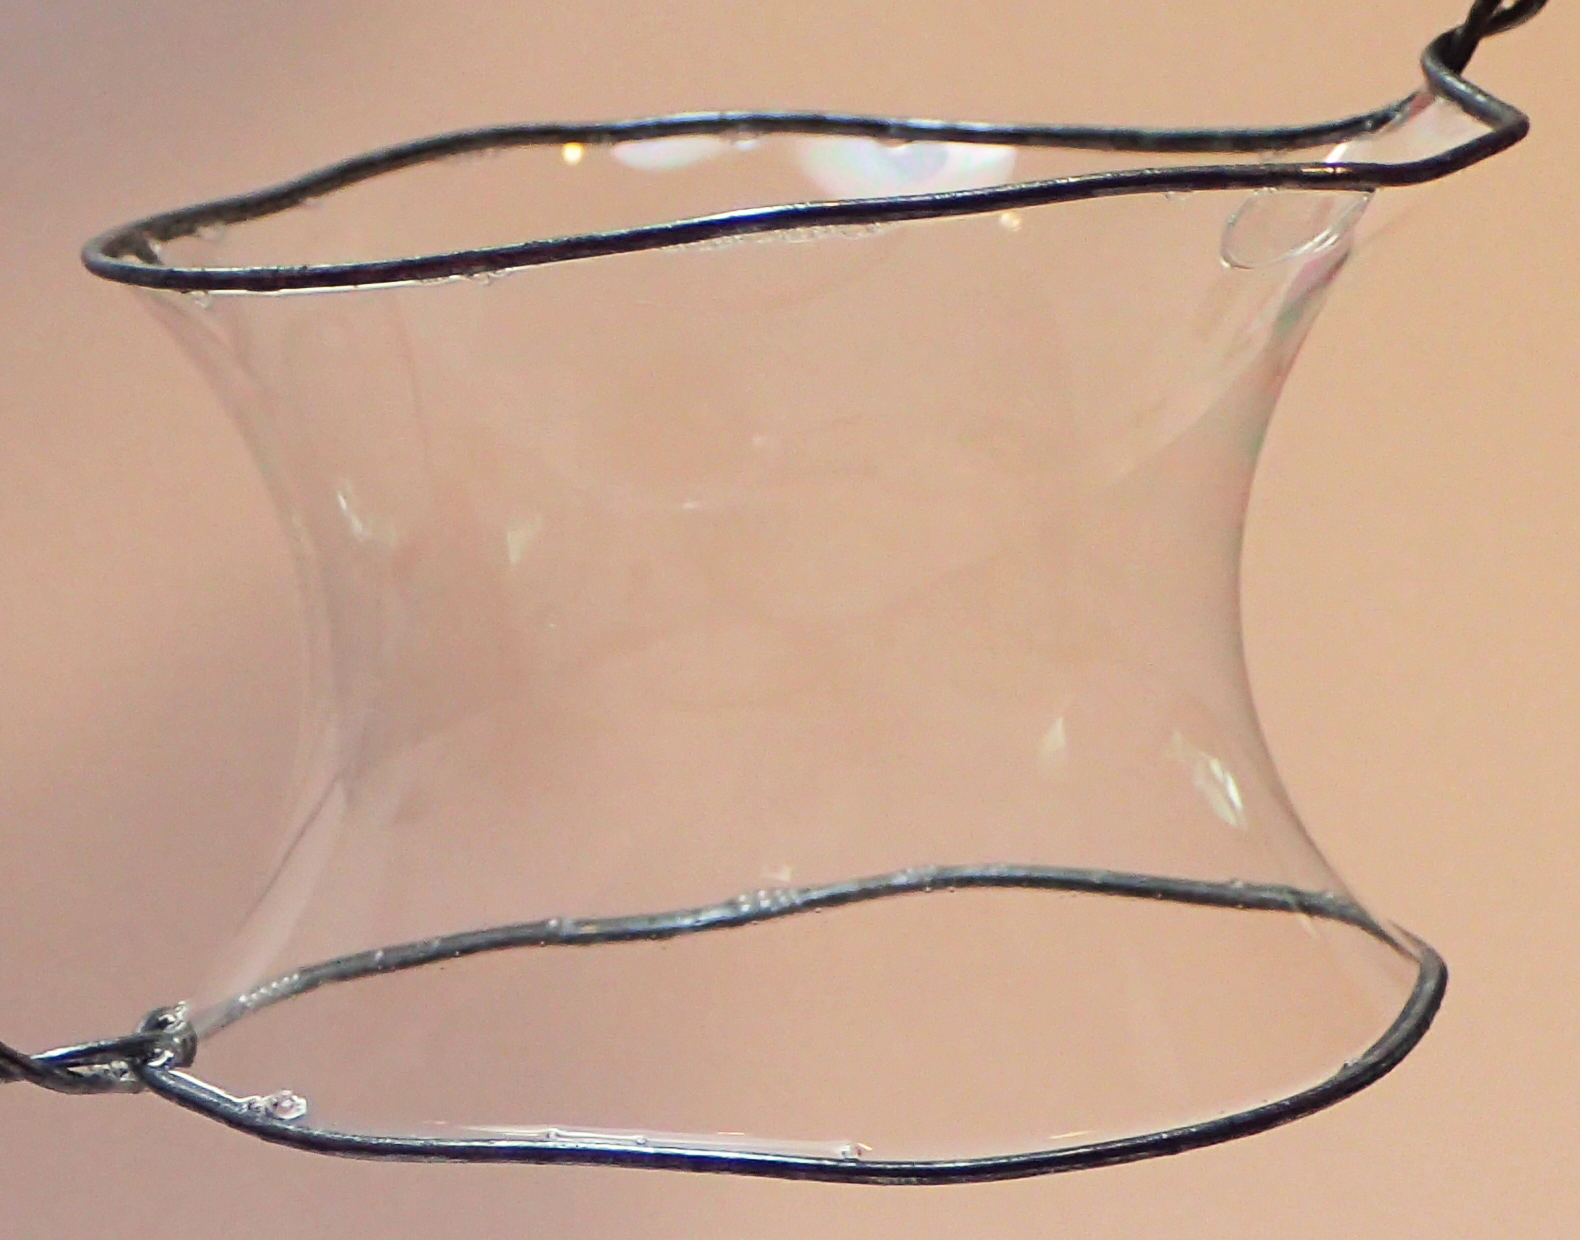
\includegraphics[scale=0.5]{minimal/Cartenoid_Foto.png}
  \caption{Seifenfilm Katenoid} 
  \label{KatenoidSeifenfilm}
\end{figure}


\begin{figure}
  \centering
  \includegraphics[scale=0.3]{minimal/Catenoid34Black.pdf}
  \caption{Skizze Katenoid} 
  \label{Katenoid}
\end{figure}
In der Skizze ~\ref{Katenoid} ist ein Katenoid abgebildet, bei welchem in Bezug auf die $z$ Achse, der untere Drahtring bei $-L$ und der obere bei $+L$ ist. 
Die beiden Kreise sollen die gleichen Radien haben, also gilt $r(-L)=r(+L)=R$. 
Mathematisch werden die Flächenpunkte des Katenoids mit der Funktion $r(z)$ beschrieben, diese wird um die Rotationsachse $z$ rotiert um den Flächeninhalt des Katenoids zu berechnen.
Hierzu braucht man eine Gleichung, welche eine Länge auf der Katenoidoberfläche beschreibt. 
Mit Hilfe Satzes von Pythagoras (Abbildung \ref{Katenoid}) kann man schreiben $ds^2=dz^2+dr^2$.
Formt man diese Gleichung um, erhält man die Gleichung

\begin{equation} \label{ds}
  ds=\sqrt{dz^2\bigg(1+\frac{dr^2}{dz^2}\bigg)}= \sqrt{dz^2(1+\dot r^2)}=\sqrt{(1+\dot r^2)}\,dz
\end{equation}
\subsubsection{Minimalfläche}
Der Seifenfilm bewegt sich automatisch in den minimalenergetischen Zustand. 
In diesem Zustand ist dann auch der Flächeninhalt $S$ des Seifenfilms minimal.
Demzufolge muss das Integral 
\begin{equation} \label{S1}  
  S= \int 2 \pi r \,ds 
\end{equation}
minimiert werden. 
Durch Einsetzen von Gleichung \eqref{ds} erhält man die Gleichung 
\begin{equation} \label{S2}
  S=2 \pi \int_{-L}^{+L} r\sqrt{1+\dot r^2}\,dz =2 \pi \int_{-L}^{+L}  F(r,\dot r, z) \,dz 
\end{equation}
welche man als Funktion $F(r,\dot r, z) = r \sqrt{1+\dot r^2}$ noch verallgemeinert schreiben kann.



Um dieses Integral \eqref{S2} zu minimieren kann man sich der Eulerschen Differenzialgleichung der Variationsrechnung bedienen. 
\subsubsection{Variationsrechnung}
Die Eulerschen Differenzialgleichung der Variationsrechnung wird im Kapitel der Geodäten \ref{skript:geodaeten:section:variationsprinzip} genauer erklärt.
Das Anwendungsprinzip wird hier kurz zusammengefasst. Hat man ein kompliziertes Integral, kann man die Eulersche Differentialgleichung anwenden, um die Extremwerte zu bestimmen. Diese besagt, dass anstelle des Ausrechnens  einer Integralfunktion der Art \begin{equation} \label{E_DGL1}  
  I(y)= \int_a^b F(x,y(x),\dot y(x))\,dx       
\end{equation}
kann auch die Differentialgleichung  



\begin{equation} \label{E_DGL2}
\bigg(\frac{\partial F}{\partial y}\bigg)- \frac{d}{dx} \bigg(\frac{\partial F}{\partial \dot{y}}\bigg)=0         
\end{equation}
gelöst werden, um die Extremwerte eines solchen Integrals zu finden.

Für die Gleichung \eqref{S2} des Flächeninhaltes des Katenoids  erhält man somit die Differentialgleichung
\begin{equation} \label{K_DGL1}
\bigg(\frac{\partial F}{\partial r}\bigg)- \frac{d}{dz} \bigg(\frac{\partial F}{\partial \dot{r}}\bigg)=0    
\end{equation}

Setzt man F ein, erhält man
\begin{equation} \label{K_DGL_H}
\sqrt{1+{\dot {r}}^2}-\frac{ d }{ dz } \bigg( r \frac{ 1 }{2  }\left( {1+{\dot {r}}^2}  \right)^{-1/2} 2 \dot {r}\bigg)=0
\\
\end{equation}
Dies wird nun schrittweise umgeformt zunächst durch ausrechnen der Ableitung

\begin{equation} \label{K_DGL_H2}
\left(1+{\dot {r}}^2  \right)^{-1/2}-\bigg(r \frac{ -1 }{2  } \left({1+{\dot {r}}^2}  \right)^{-3/2} 2 \dot{r} \ddot{r}  \dot{r}+ r \left({1+{\dot {r}}^2}  \right)^{-1/2} \ddot{r} +\dot{r} \left({1+{\dot {r}}^2}  \right)^{-1/2} \dot{r}\bigg)=0
\end{equation}
bis die Differentialgleichung zweiter Ordnung  
\begin{equation} \label{K_DGL_R}
1+{\dot {r}}^2=r  \ddot{r}
\end{equation}
entsteht. 
Gesucht ist also eine Funktion $r(z)$, die die Differentialgleichung \eqref{K_DGL_R} erfüllt. Als Randbedingungen für die Funktion $r(z)$ sind in diesem Beispiel $r(+L)=R$ und $r(-L)=R$ aus der Abbildung \ref{Katenoid} gegeben.

\subsubsection{Lösen der Differentialgleichung}
Die Differenzialgleichung zweiter Ordnung \eqref{K_r} kann mit Hilfe einiger mathematischer Umformungen, Aufleiten und hyperbolischer Trigonometrie gelöst werden. 
Dies ist eine langwierige Berechnung und wird daher hier nicht durchgeführt.

Anstelle des konkreten Ausrechnens kann man die Lösung der Differentialgleichung \eqref{K_DGL_R} auch erraten. 
Aus der hyperbolischen Trigonometrie ist $\cosh^2-\sinh^2=1$ oder anders geschrieben $1+\sinh^2=\cosh^2$ \eqref{K_hTrigo} bekannt. 
Beim Ableiten von $\cosh$ erhält man $\sinh$ und $\sinh$ abgeleitet ergibt wieder $\cosh$. 
Mit dieser Erkenntnis kann man durch das Vergleichen der Gleichungen versuchen die Form der Lösung der DGL \eqref{K_DGL_R2} zu erraten. 

Der Term $\sinh^2$  (zweiter Term links) soll der quadrierten Ableitung einer Funktion ${\dot {r}}^2$ entsprechen also kann man schreiben $(\cosh)'^2$. 
Auf der rechten Seite sollte $\cosh^2=\cosh \cosh$ dem Produkt von einer Funktion und ihrer doppelten Ableitung gleich kommen. Da gilt $(\cosh)''=(\sinh)'=\cosh$, kann die rechte Seite so $(\cosh) (\cosh)''$ auch durch $\cosh$ ausgedrückt werden.


Zusammengefasst kann man die Gleichung 
\begin{equation} \label{K_hTrigo}
1+\sinh^2=\cosh^2
\end{equation}
 in die Gleichung 
 \begin{equation} \label{K_DGL_R2}
1+{\dot {r}}^2=r  \ddot{r}
\end{equation}
 umformen und sieht mit Hilfe der Gleichung 
\begin{equation} \label{K_hTrigoU}
1+(\cosh)'^2=(\cosh) (\cosh)''
\end{equation}
dass $r(z)$ eine Funktion in $\cosh$ sein muss.
Die exakte Lösung der Differentialgleichung \eqref{K_DGL_R} beinhaltet noch die zwei Konstanten $K$ und $\xi$, welche durch die doppelte Integration dazukommen. Daraus resultiert somit für $r(z)$ die Gleichung 

\begin{equation} \label{K_r}
r(z)=K \cosh\bigg(\frac{z-\xi}{K}\bigg)
\end{equation}

Unter Einbezug der Anfangsbedingungen $r(+L)=R$ und $r(-L)=R$, aus Abbildung \ref{Katenoid}, ist der Radius $R$ bei $z= \pm L$ gleich gross. Deshalb kann man $r(+L)$ mit $r(+L)$ und $R$ gleichsetzen. Durch einsetzen der Funktion $r(z)$ erhält man folglich die Gleichung
\begin{equation} \label{K_rL}
K \cosh\bigg(\frac{L-\xi}{K}\bigg)=K \cosh\bigg(\frac{-L-\xi}{K}\bigg)=R
\end{equation}

Da der $\cosh$ eine gerade Funktion ist, kommt man entweder auf $L-\xi=-L-\xi$ oder auf $L-\xi=-(-L-\xi)$. Die Integrationskonstante $K$ kann bei diesen zwei Gleichungen für $L$ weggelassen werden, da eine beidseitige Division bei den Gleichungen überflüssig ist.
Beim ersten Fall wäre $L=-L$, was keinen Sinn ergibt, da dann $L=0$ wäre. Beim zweiten Fall muss $\xi=0$ sein, also ist die Lösung für das Katenoid die Funktionsgleichung 

\begin{equation} \label{K_rz}
r(z)=K \cosh\left(\frac{z}{K}\right)
\end{equation}
mit $z$ als Parameter und $K$ als Integrationskonstante.
\section{Sattelfläche}
\rhead{Sattelfläche}
Es gibt mehrere verschiedene Arten Minimalflächen zu Charakterisieren, das Beispiel des Katenoids illustriert das Konzept des minimalen Flächeninhaltes. 
Eine mathematischere Definition basiert auf der mittleren Krümmung. 
In diesem Buch wurde bis anhin hauptsächlich die Gauss Krümmung betrachtet. 
Dies weil wir uns auf der Erde in (oder direkt auf) der zu Betrachtenden Fläche befinden. 
Anders formuliert, ist die Gausskrümmung ein Mass für die innere Krümmung einer Fläche, der Fachbegriff für diese Art Krümmung ist intrinsische Krümmung. 
Die mittlere Krümmung im Gegenzug ist eine extrinsische Krümmung, was heisst, dass der Beobachter von aussen die Krümmung der Fläche beobachtet.
Folgend wird zuerst das Konzept der Krümmung kurz zusammengefasst und anschliessend der Unterschied der mittleren und Gauss Krümmung im Bezug auf Minimalflächen illustriert, bevor dies alles mit dem Beispiel der Sattelfläche visualisiert wird.


\subsection{Krümmung einer Fläche}
\index{Krümmung einer Fläche}

Intuitiv ist Krümmung einer Fläche für uns ein Mass der Abweichung eines Objekts im Bezug zu einer Ebene. 

Die Krümmung einer Fläche im Punkt $P$ kann in der Mathematik indirekt durch die Hauptkrümmungsradien $R_1$ und $R_2$ ausgedrückt werden. 
Die Hauptkrümmungsradien hängen von den Tangentenrichtungen im Punkt P ab. 
Die Tangentenrichtungen stehen senkrecht aufeinander.
Sie sind so definiert, dass $R_1$ den Minimalwert und $R_2$ den Maximalwert annimmt.

Unter dem Krümmungsradius versteht man den Radius des Kreises, welcher die Kurve im Punkt $P$ am besten approximiert. 
Da wir intuitiv bei einem Kreis oder einer Kugel eine grosse Krümmungszahl erwarten und bei einer fast ebenen Fläche eine kleine, ist die Krümmung $k$  als der Kehrwert des Krümmungsradius definiert $k=1/R$ . 

\begin{figure} 
  \centering
  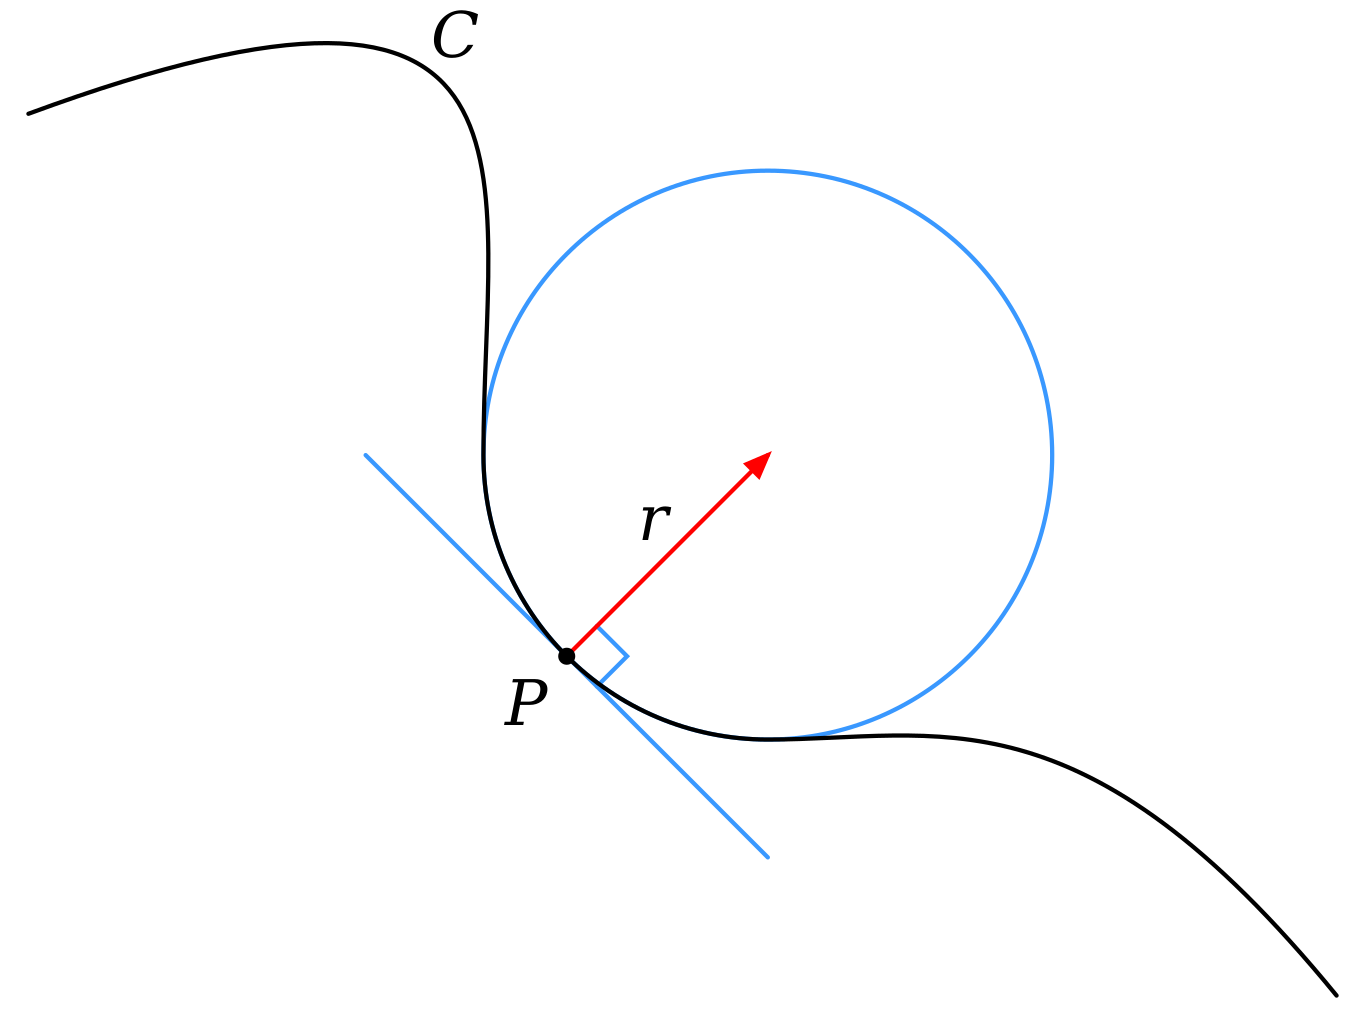
\includegraphics[scale=0.1]{minimal/Kruemmungsradius.png}
  \caption{Krümmungsradius} 
\end{figure}

Überträgt man das Konzept der Krümmung ins Dreidimensionale braucht es zwei Krümmungen, welche orthogonal zueinander stehen, um die Krümmung an einem Punkt zu bestimmen. Diese werden als Hauptkrümmungen $k_1$ und $k_2$ bezeichnet.
Zur nummerischen Charakterisierung der Krümmung einer Fläche in der Mathematik werden hauptsächlich zwei Grössen benutzt.
Zum einen die Gauss Krümmung, welche eine intrinsische Krümmung ist und zum andern die mittlere Krümmung bei welcher es sich um eine extrinsische Krümmung handelt. Bei Minimalflächen ist vor allem die mittlere Krümmung von Bedeutung.


\index{Gauss Krümmung}
\subsubsection{Gauss Krümmung}
Die Gauss Krümmung einer Fläche im Punkt $P$ ist definiert als das Produkt der zwei Hauptkrümmungen $k_1$ und $k_2$.

\begin{equation} \label{Gauss_Kruemmung_D}
  H=k_1\, k_2= \frac{1}{R_1}\frac{1}{R_2}
\end{equation}



Die Gauss Krümmung ist eine intrinsische Krümmung. Diese ist  ein Mass für die innere Krümmung einer Fläche. 
Eine gute Vorstellungshilfe ist die Ameisenperspektive. 
Wenn die Ameise auf einer Kugel ist kann sie feststellen, dass nur schon in ihrem kleinen Blickfeld die Winkelsummen eines Dreiecks auf der Oberfläche grösser als 180° ist, demzufolge besitzt die Kugel eine positive Gauss Krümmung. Anders sieht es aus bei einem Zylinder dort misst die Ameise auf der Zylinderoberfläche genau 180° Winkelsumme, dass heisst die Gauss Krümmung eines Zylinders ist null.

\index{mittlere Krümmung}
\subsubsection{Mittlere Krümmung}
Die mittlere Krümmung einer Fläche im Punkt $P$ ist definiert durch den Mittelwert der zwei Hauptkrümmungen $k_1$ und $k_2$.

\begin{equation} \label{Mittlere Kruemmung_D}
  H=\frac{1}{2}(k_1+k_2)= \frac{1}{2}\bigg(\frac{1}{R_1}+\frac{1}{R_2}\bigg)
\end{equation}

Die mittlere Krümmung ist eine extrinsische Krümmung. 
Im Gegensatz zur intrinsischen Krümmung kommt es bei einer extrinsischen Krümmung auf die Umgebung an. 
Man kann sich vorstellen, dass man zum Beispiel die Krümmung eines Zylinders (zweidimensionales Objekt) von aussen, also in einem dreidimensionalen Raum betrachtet. 
Ein Zylinder ist aus der Ameisenperspektive flach, schaut man von aussen, sieht er jedoch gekrümmt aus.
Dies, weil er eine positive mittlere Krümmung aufweist. 
Anders sieht es zum Beispiel bei einer Sattelfläche (Pringels-Chips artigen Fläche) aus, dort ist die Gausskrümmung negativ, hingegen kann die mittlere Krümmung im Spezialfall, dass $R_1=-R_2$, also die Krümmungsradien ein umgekehrtes Vorzeichen aufweisen, aber vom Betrag her identisch sind, gleich null sein. 
In diesem Fall ist diese Sattelfläche ein Beispiel für eine Minimalfläche.
Die besondere Bedeutung der mittleren Krümmung H besteht darin, dass Minimalflächen dadurch charakterisiert sind, dass für sie gilt $H=0$. Im Abschnitt \ref{Young-Laplace} wird die Young-Laplace-Gleichung hergeleitet, welche erklärt warum Minimalflächen die Eigenschaft $H=0$ haben. Der Beweis, dass die mittlere Krümmung bei Minimalflächen gleich null sein muss, übersteigt jedoch den Umfang dieses Kapitels er kann bei Interesse in der Literatur \ref{minimal:MotionOfSurfaceByItsMeanCurvature} nachgelesen werden. 

\begin{figure} 
  \centering
  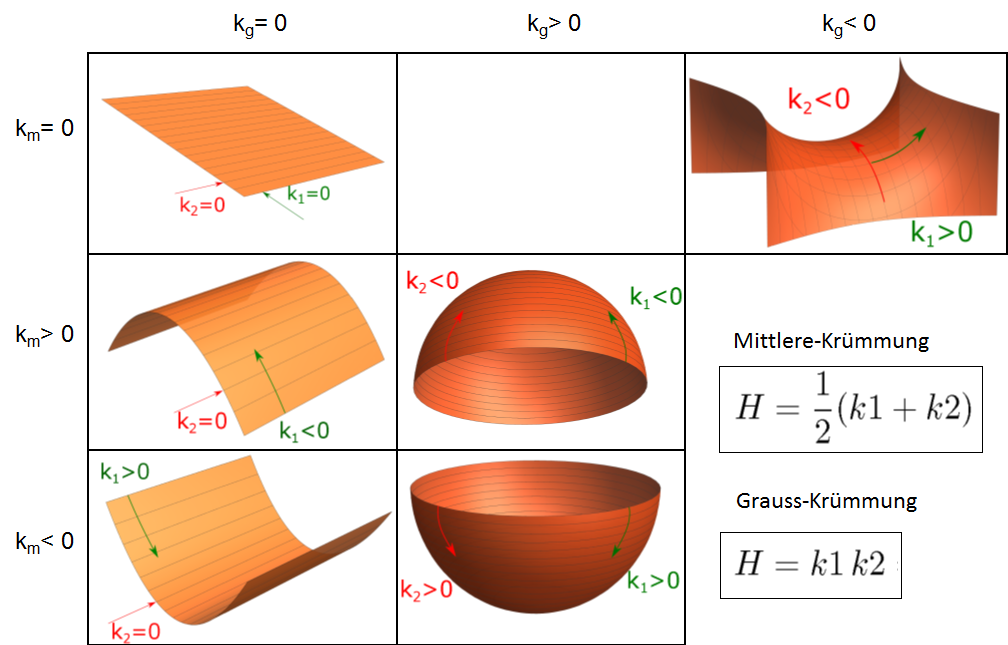
\includegraphics[scale=0.4]{minimal/Tabelle_Kruemmung.png}
  \caption{Vergleich Grauss und Mittlerkrümmung} 
\end{figure}



\subsection{Beispiel Scherksche Sattelfläche}
\begin{figure}
  \centering
  \includegraphics[scale=0.2]{minimal/HFSherckV2.pdf}
  \caption{Sattelfläche von Scherk} 
  \label{fig:Scherk}
\end{figure}
Eine Scherksche Sattelfläche \. (Abbildung: \ref{fig:Scherk})\, ist eine Fläche, deren Gausskrümmung, wie bei jeder Sattelfläche, kleiner als null ist und zusätzlich eine mittlere Krümmung von genau null hat. Dies bedeutet, dass in jedem Punkt der Fläche die Krümmungen vom Betrag her gleich sind, aber ein umgekehrtes Vorzeichen haben. 


Eine Approximation an die Fläche kann mittels Drahtgeflecht und einer Seifenlösung nachgebildet werden \. (Abbildung: \ref{fig:SoapScherk}). Die einzelnen Seifenmoleküle versuchen ein stabiles Gleichgewicht der abstossenden und anziehenden Kräfte zu finden. Dieser stabile Punkt braucht durch das Gleichgewicht ein Minimum an Energie. Dies bedeutet auch, dass die Krümmung, welche Energie benötigt, minimiert wird.
\begin{figure}
  \centering
  \includegraphics[scale=0.3]{minimal/SattelflacheSoapFilm.png}
  \caption{Seifenfilm bildet Minimalfläche} 
  \label{fig:SoapScherk}
\end{figure}
Die Sattelfläche wurde erstmals 1834 von Prof. H. F. Scherk beschrieben cite{minimal:JournalAM} und hergeleitet. Sie war nach der in 1776 von Meusnier beschriebene Katanoide die erste neue Minimalfläche. Im folgenden Abschnitt, wird die Gleichung mittels Minimalflächengleichung (im Englischen unter dem Namen Minimal Surface Equation bekannt) cite{minimal:Gray} berechnet. 

Die Minimalflächengleichung ist eine partielle Differentialgleichung welche durch Lösen der Euler-Lagrange Gleichung \ref{skript:geodaeten:subsection:Euler-Lagrange-Gleichung} für Flächen mit mittlerer Krümmung $M=0$ gefunden wird. Das lösen dieser würde den Rahmen hier aber deutlich übersteigen. 

\subsubsection{Lösen der Partiellen Differentialgleichung}\label{Scherk Berechnung}
Angenommen $z=Z(x,y)$ ist die Funktion eines Graphen. Wobei ${x,y}$ die Koordinaten in der Ebene sind, welche nach $z$ Abgebildet werden. Gesucht werden alle Lösungen welche sich als $z=Z(x,y)=f(x)+g(y)$ schreiben lassen und die Bedingungen $Z(0,0)=0,\ \nabla Z(0,0)=0$ erfüllen.

$Z_x$ ist die erste Ableitung der Funktion $Z(x,y)$ nach $x$. $Z_y$ ist äquivalent dazu die erste Ableitung der Funktion $Z(x,y)$ nach $y$. $Z_{xx}$ und $Z_{yy}$ sind die jeweils 2. Ableitungen der Funktion $Z(x,y)$ nach den entsprechenden Indizes. $Z_{xy}$ ist die Ableitung von $Z_x$ nach $y$. Beziehungsweise die Funktion $Z(x,y)$ erst nach $x$ und dann zusätzlich nach $y$ abgeleitet. 

Wir nutzen die Minimalflächengleichung
\begin{equation}\label{Minimalflaechengleichung}
(1+ Z_x^{2})Z_{xx} - 2 Z_x Z_y Z_{xy} + (1+ Z_x^{2}) Z_{yy}=0
\end{equation}
und setzen die Ableitungen und mehrfachen Ableitungen der Funktion $Z(x,y)$ ein. Da $ Z_x = f'(x),\ Z_y = g'(y),\ Z_{xx}=f''(x),\ Z_{yy} = g''(y) \ \text{und} \ Z_{xy}=0$ ist, vereinfacht sich die Minimalflächengleichung zu 
\begin{equation}\label{MFG Scherk}
(1+g'(y)^2)f''(x)+(1+f'(x)^2)g''(y)=0
\end{equation}
Durch Separieren von $f$ und $g$ stellt sich die Gleichung folglich auf
\begin{equation}\label{MFG Scherk2}
-\dfrac{f''(x)}{1+(f'(x))^2}=\dfrac{g''(y)}{1+(g'(y))^2}=c
\end{equation}
mit $c \in \mathbb{R}$ konstant. $c$ ist Konstant, da die Gleichung nur stimmen kann, wenn trotz unterschiedlichen Variablen $x$ und $y$ beide Quotienten bei einer Veränderung in $x$- beziehungsweise $y$-Richtung gleich bleiben. Wird zum Beispiel $x=0$ fixiert und $y$ variiert muss die Differentialgleichung in $g(y)$ konstant bleiben, da sonst die Gleichung durch die Veränderung des 2. Quotienten ungleich wäre.\\
Die Differenzialgleichungen in $f$ und $g$ werden nun separat gelöst. Erst wird $f'(x)$ mit $w(x)$ substituiert. Anschliessend wird die Gleichung  beidseitig integriert und nach $w(x)$ aufgelöst.
\begin{equation}\label{ScherkDGL1}
\begin{split}
\int -\dfrac{w'(x)}{1+w(x)^2} dx &= \int c \ dx , \quad w(x)=f'(x) \\
-\arctan(w(x)) &= cx+k_1 \\
w(x) &= -\tan(cx+k_1)
\end{split}
\end{equation}
Nach der Rücksubstitution wird nochmals auf beiden Seiten integriert:
\begin{equation}\label{SchreckDGL2}
\int f'(x)\ dx = \int -\tan(cx+k_1)\ dx\\
\end{equation}
\begin{equation}
f(x) = \dfrac{\log(\cos(cx+k_1))}{c}+k_2\\
\end{equation}
mit $f(0)=0$ und $f'(0)=0$ ergibt sich
\begin{equation}
f(x) = \dfrac{\log(\cos(cx))}{c}\\
\end{equation}
Äquivalent dazu ergibt sich für die 2. Differenzialgleichung:
\begin{equation}
g(y) = - \dfrac{\log(\cos(cx))}{c}
\end{equation}
Somit lautet die Funktion der Scherkschen Minimalfläche
\begin{equation}
Z(x,y)=\dfrac{\log(\cos(cx))}{c}-\dfrac{\log(\cos(cy))}{c}.
\end{equation}

\subsection{Beispiel Young–Laplace - Oberflächenspannung}
\rhead{Young–Laplace}
\label{Young-Laplace}

\label{YL-Beschreibung}
In den vorangegangenen Beispielen wurde jeweils eine Lösung gesucht, bei der die Mittlere Krümmung $H=0$ ist. Bei den meisten Oberflächen ist dies jedoch nicht der Fall. Beispielsweise haben Seifenblasen innen und aussen einen anderen Druck. Oder in einem Blutgefäss herrscht innen der Blutdruck und außerhalb der Druck durch die Gewebe.

Dennoch haben solche Oberflächen ähnliche Eigenschaften, da auch hier die Energie minimiert wird. Dies wird durch die Young-Laplace Gleichung \cite{minimal:Laplace} beschrieben, welche im folgenden Abschnitt mittels geometrischen und physikalischen Überlegungen hergeleitet wird.
\subsubsection{Herleitung der Young-Laplace Gleichung}\label{YL-Herleitung}
Angenommen zwei Medien (z.B. Luft/Wasser) werden durch eine Oberfläche \. (Abbildung: \ref{fig:YoungCone}) getrennt. Da in den Medien verschiedene Drücke $p_1$ und $p_2$ herrschen, wölbt sich die Oberfläche. Die Veränderung des Krümmungsradius sei $\delta\zeta$ \.(Abbildung: \ref{fig:Strahlensatz}). Das Volumen eines einzelnen infinitesimalen Volumensegments sei $\delta\zeta\,dA$ \.(Abbildung: \ref{fig:Volumentransaltion}). Dann ist die benötigte Kraft um das Volumensegment um $\delta\zeta$ zu verschieben:
\begin{figure}
  \centering
  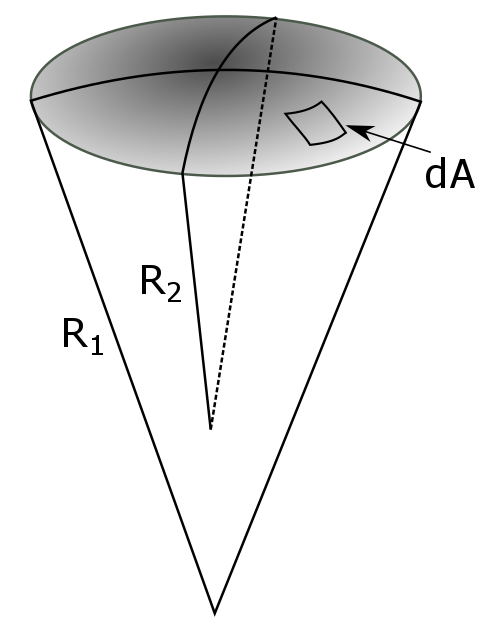
\includegraphics[scale=0.3]{minimal/YoungCone.png}
  \caption{Ausschnitt aus einer Oberfläche mit Krümmungsradien} 
  \label{fig:YoungCone}
\end{figure}
\begin{figure}
  \centering
  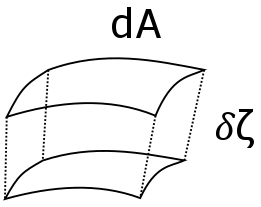
\includegraphics[scale=0.3]{minimal/Volumetranslation.png}
  \caption{Element der Volumentranslation} 
  \label{fig:Volumentransaltion}
\end{figure}
\begin{equation}
\delta W=\int(-p_1+p_2)\,\delta\zeta\,dA
\end{equation}
Die Gesamte Arbeit ergibt sich, wenn zur Arbeit der Volumenänderung die Arbeit der Veränderung der Oberfläche $\delta W=\gamma \, \delta A $ dazu addiert wird, wobei $\gamma$ die Oberflächenspannung und $\delta A$ die veränderte Oberfläche ist. Wir erhalten:
\begin{equation}\label{YL-Arbeit_1}
\delta W=\int(-p_1+p_2)\,\delta\zeta dA + \gamma \,\delta A
\end{equation}
Sind $R_1$ und $R_2$ die Krümmungsradien der Oberfläche, werden die infinitesimalen Längenstücke $dl_1$ und $dl_2$ bei einer Veränderung der Radien $R$ um $\delta\zeta$ mittels Strahlensatz \.(Abbildung: \ref{fig:Strahlensatz})
\begin{equation}
\frac{R}{dl}=\frac{R+\delta\zeta}{dl+x}
\end{equation}
verlängert. Wobei $dl+x=dl'$ ist. Nach $dl'$ umgeformt ergibt sich
\begin{equation}
dl' = dl(\frac{R+\delta\zeta}{R})
\end{equation}
durch einfache Umformungen erhalten wir
\begin{equation}
\begin{split}
dl' &= dl(1+\frac{\delta\zeta}{R})\\
&=dl+\frac{dl\,\delta\zeta}{R}
\end{split}
\end{equation}
\begin{figure}
  \centering
  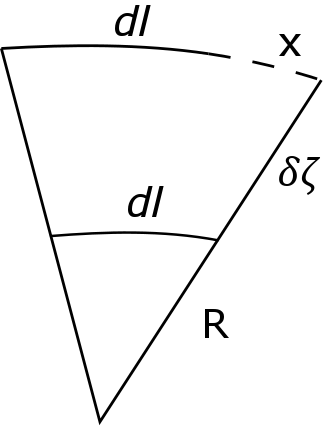
\includegraphics[scale=0.3]{minimal/Langenanderung.png}
  \caption{Längenänderung} 
  \label{fig:Strahlensatz}
\end{figure}
Das Flächenstück $dA=dl_1 dl_2$ verändert sich somit
\begin{equation}
\begin{split}
dA' &= (1+\frac{\delta\zeta}{R_1})\, dl_1 (1+\frac{\delta\zeta}{R_2}) \, dl_2 \\
&\approx dl_1\,dl_2\,(1+\frac{\delta\zeta}{R_1} + \frac{\delta\zeta}{R_2})
\end{split}
\end{equation} 
Somit ist die Änderung eines Flächenstück $\delta dA=dA'-dA$
\begin{equation}
\begin{split}
\delta dA &= dl_1\,dl_2\,\delta\zeta\,(1+\frac{1}{R_1}+\frac{1}{R_2})-dl_1\,dl_2\\
\delta dA &= dl_1\,dl_2\,\delta\zeta\,(\frac{1}{R_1}+\frac{1}{R_2})
\end{split}
\end{equation}
Die veränderte Oberfläche kann damit berechnet und in die Gleichung \ref{YL-Arbeit_1} eingesetzt werden. 
\begin{equation}
\delta A = \int \delta\zeta \, \bigg( \frac{1}{R_1}+\frac{1}{R_2} \bigg)\,dA \\
\end{equation}
Befindet sich die Oberfläche im Gleichgewicht, muss auch die Variation der Arbeit gleich Null sein.
\begin{equation}
\delta W = \int \delta\zeta \, \bigg[ (-p_1+p_2)-\gamma \, \bigg( \frac{1}{R_1}+\frac{1}{R_2} \bigg) \bigg]\,dA =0
\end{equation}
Da $\delta\zeta=0$ eine triviale Lösung wäre, ist $\delta\zeta \neq 0$. Daraus folgt die endgültige Formel:
\begin{equation}
-p_1+p_2 = \gamma \, \bigg( \frac{1}{R_1}+\frac{1}{R_2} \bigg)
\end{equation}
oder
\begin{equation}\label{Young-Laplace}
\Delta p = \gamma \, \bigg( \frac{1}{R_1}+\frac{1}{R_2} \bigg)
\end{equation}
Mithilfe dieser Formel kann auch gezeigt werden, dass eine klassische Seifenblase keine Minimalfläche ist. Nehmen wir an, dass eine Seifenblase im freien Fall (z.B. in der ISS) kugelförmig ist und eine Oberflächenspannung $\gamma$ von $\frac{1}{2}$ hat, vereinfacht sich die Young-Laplace Gleichung
\begin{equation}\label{eq:Sphere}
\begin{split}
\Delta p = \frac{1}{2}(\frac{1}{r}+\frac{1}{r}) \\
\end{split}
\end{equation}
zu
\begin{equation}
\begin{split}
\Delta p &= \frac{1}{2}(\frac{2}{r})\\
\Delta p &=\frac{1}{r}.
\end{split}
\end{equation}
Es ist leicht ersichtlich, dass die Young-Laplace Gleichung \ref{eq:Sphere} der Gleichung der mittleren Krümmung \ref{Mittlere Kruemmung_D} ähnelt. Damit die Kugel einer Minimalfläche entspräche müsste die Gleichung 0 ergeben. Dies wäre aber erst bei einem unendlichen Radius der Fall. 



\printbibliography[heading=subbibliography]
\end{refsection}